\chapter{}
In der Vorlesung geht es um die Einführung der Initialen Topologien
-Ich denke das es darum geht anhand von dem was mein Auge erblickt-

\section{Kommutative Diagramme zur Veranschaulichung}

Weil die Konstrucktion bei einem normalen (Auch bei nicht normalen) menschen
ein paar knoten im kopf verursacht, wollen wir uns das ganze mal 
mit Bildern anschauen (Kommutative Diagramme).\\
Seien $X_i, i\in I$ Mengen "mit Topologien" und 
$
\Phi:
\begin{cases} Y\to \prod_{i\in I}X_i\\
    (\alpha_i(y))_{i\in I} \mapsto X_i
\end{cases}
$
eine Abbildung.\\
Wobei $\alpha_{i}: \pi_i \circ \Phi,  \forall i \in I$  mit $\pi_i$
die Projektion auf die $i$-te Komponente ist und damit ist $\pi_i$ stetig     
$\forall i \in I$.\\

\begin{tikzpicture}[>=stealth, xscale=1.2, yscale=1.2]

% X oben
\node (Y) at (0,0) {$Y$};

% Xi und Xj darunter
\node (Xi) at (0,-2) {$\prod_{i\in I}X_i$};

% Zielräume ganz unten (4 Stück)
\node (Xk-1) at (-4,-4) {$(X_{k-1},\mathcal{T}_{k-1})$,};
\node (dots) at (-3,-4) {\quad$\dots$,};
\node (Xk) at (-2,-4) {$(X_{k},\mathcal{T}_{k})$,};
\node (X0) at (0,-4) {$\dots$};
\node (Xj) at (2,-4) {,$(X_{j},\mathcal{T}_{j})$,};
\node (dots2) at (3,-4) {$\dots$,};
\node (Xj+1) at (4,-4) {\quad ,$(X_{j+1},\mathcal{T}_{j+1})$};

% f_i, f_j
\draw[->, dashed] (Y) -- node[left] {$\Phi$} (Xi);

% Xi → Ziele
\draw[->] (Xi) -- node[left] {$\pi_{k}$} (Xk);
\draw[->] (Xi) -- node[right] {$\pi_{j}$} (Xj);

% gestrichelte Kompositionen
\draw[->] (Y) .. controls (-2,-1) .. node[left] {$\alpha_{k}$} (Xk);
\draw[->] (Y) .. controls (2,-1) .. node[right] {$\alpha_{j}$} (Xj);

\end{tikzpicture}

Davon ausgehend wollen wir eine Topologie auf $Y$ definieren, die sogenannte \textbf{initiale Topologie} 
bezüglich der Familie von Abbildungen $(\alpha_i)_{i\in I}$.\\
 

\begin{tikzpicture}[>=stealth, xscale=1.2, yscale=1.2]

% X oben
\node (Y) at (0,0) {$\langle Y,\mathcal{V}\rangle$};

% Xi und Xj darunter
\node (Xi) at (0,-2) {$\langle \prod_{i\in I}X_i,\prod_{i\in I}\mathcal{T}_i \rangle$};

% Zielräume ganz unten (4 Stück)
\node (Xk-1) at (-4,-4) {$\langle X_{k-1},\mathcal{T}_{k-1}\rangle$,};
\node (dots) at (-3,-4) {\quad$\dots$,};
\node (Xk) at (-2,-4) {$\langle X_{k},\mathcal{T}_{k}\rangle$,};
\node (X0) at (0,-4) {$\dots$};
\node (Xj) at (2,-4) {,$\langle X_{j},\mathcal{T}_{j}\rangle$,};
\node (dots2) at (3,-4) {$\dots$,};
\node (Xj+1) at (4,-4) {\quad ,$\langle X_{j+1},\mathcal{T}_{j+1}\rangle$};

% f_i, f_j
\draw[->, dashed] (Y) -- node[left] {$\Phi$} (Xi);

% Xi → Ziele
\draw[->] (Xi) -- node[left] {$\pi_{k}$} (Xk);
\draw[->] (Xi) -- node[right] {$\pi_{j}$} (Xj);

% gestrichelte Kompositionen
\draw[->] (Y) .. controls (-2,-1) .. node[left] {$\alpha_{k}$} (Xk);
\draw[->] (Y) .. controls (2,-1) .. node[right] {$\alpha_{j}$} (Xj);

\end{tikzpicture}

\nt{
    $\prod_{i \in I} \mathcal{T}_i$ ist die Kleinste Topologie mit 
    $$\bigcup_{i \in I}\{\pi^{-1}(O_i)\mid \mathcal{O}_i \in \mathcal{T}_i\}$$
}
\section{Konstrucktion ohne Zeichnen}

Im folgenden wollen wir zeigen das wenn gilt: 
Seien $X_i, i \in I$ Mengen mit Topologien $\mathcal{T}_i$ und 
$\alpha_{i}: \pi_i \circ \Phi \forall i \in I$ und $\pi_i$ stetig $\forall i \in I$
Dann ist $\Phi$ stetig

\dfn{
    Seien $\rangle X_i,\mathcal{T}_i \langle, i \in I$ topologische, $i \in I$
    $X$ eine Menge und $f_i: X \to X_i$ Abbildungen, $\forall i \in I$.
    Die \textbf{initiale Topologie} $\mathcal{T_{\text{init}}}$ auf $X$ bezüglich der Familie von Abbildungen 
    $(f_i)_{i \in I}$ ist die kleinste Topologie auf $X$, so dass alle Abbildungen $f_i$ stetig sind.   
    $$
     \mathcal{T}_{\text{init}} := \text{Topologie erzeugt von } \bigcup_{i \in I}\{f_i^{-1}(O_i) \mid O_i \in \mathcal{T}_i\} 
    $$
}

\thm{}
{
    Seien $\langle X_i,\mathcal{T}_i \rangle,  i \in I$ topologische Räume, $X$ eine Menge und 
    $f_i: X \to X_i$ Abbildungen, $\forall i \in I$. und $\mathcal{T}$ ist Topologie auf $X$.
    Dann sind die folgenden Aussagen äquivalent:
    \begin{enumerate}
        \item[(i)] $\mathcal{T} = \mathcal{T}_{\text{init}}$
        \item[(ii)] Für jeden topologischen Raum $\langle Y, \mathcal{V} \rangle$ und jede Abbildung 
        $g: \langle Y, \mathcal{V} \rangle \to \langle X, \mathcal{T} \rangle$ ist stetig genau dann, wenn alle Kompositionen 
        $f_i \circ g: \langle Y, \mathcal{V} \rangle \to \langle X_i, \mathcal{T}_i \rangle$ stetig sind, $\forall i \in I$.
    \end{enumerate}
}

\begin{proof}{Satz:11.2.2}
    \begin{enumerate}
        \item["(i) $\Rightarrow$ (ii)"] Sei $g: \langle Y, \mathcal{V} \rangle \to \langle X, \mathcal{T} \rangle$ eine Abbildung.
        \begin{itemize}
            \item ["$\Rightarrow$"] $\bigcup_{i \in I}\{f_1^{-1}\}$ ist Subbasis von $\mathcal{T}$.
            Sei also $O_i \in \mathcal{T}_i, i \in I O_i \in \mathcal{T}_i$:
            $$g^{-1}(f_i^{-1}(O_i)) = (f_i \circ g)^{-1}(O_i) \in \mathcal{V}$$
            \item["$\Leftarrow$"] $f_i: \langle X, \mathcal{T} \rangle \to \langle X_i, \mathcal{T}_i \rangle$ stetig $\forall i \in I$.
            $\Rightarrow f_i \circ g$ stetig $\forall i \in I$
        \end{itemize}
    \item["(ii) $\Rightarrow$ (i)"] 
    \begin{itemize}
        \item[(1)]
            $$
            \begin{tikzcd}[column sep=large, row sep=large]
            & \langle X, \mathcal T_{\mathrm{ini}} \rangle 
                \arrow[d, "\mathrm{id}_X"'] 
                \arrow[dr, "f_i", bend left=15] & 
                \\
            & \langle X, \mathcal T \rangle 
                \arrow[r, "f_i"'] 
            & \dots, \langle X_i, \mathcal T_i \rangle, \dots
            \\[1em]
            \text{stetig} & & \text{stetig}
            \end{tikzcd}
            \qquad
            id_X \text{ stetig wegen (ii).}
            \qquad
            (\mathcal T \subseteq \mathcal T_{ini})
            $$
        \item[(2)]
        $$
        \begin{tikzcd}[column sep=large, row sep=large]
        & \langle X, \mathcal T \rangle 
        \arrow[d, "\mathrm{id}_X"'] 
        \arrow[dr, "f_i", bend left=15] & 
        \\
        & \langle X, \mathcal T \rangle 
        \arrow[r, "f_i"'] 
        & \dots, \langle X_i, \mathcal T_i \rangle, \dots
        \\[1em]
        & \text{stetig} & \text{stetig}
        \end{tikzcd}
        $$

        $$
        \text{mit (ii) } \Rightarrow\ 
        f_i : \langle X, \mathcal T \rangle \to \langle X_i, \mathcal T_i \rangle
        \text{ stetig}
        $$

        $$
        \Rightarrow\quad
        \mathcal T \supseteq 
        \bigcup_{i\in I} \{\, f_i^{-1}(U_i) \mid U_i \in \mathcal T_i \,\}
        \Rightarrow\quad
        \mathcal T = \mathcal T_{\mathrm{ini}}.
        $$
    \end{itemize}
\end{enumerate}
\end{proof}

\thm{}
{
   
Seien  $X$ und $(X_i) i\in I $ Mengen mit Abbildungen
$f_i: X \to X_i$ für $i\in I$. Witers seine $XX_{i_\ell}$ Menten mit
$\ell \in J_i$ Abbildungen $g_{i\ell} : X_i \to X_{i\ell}$ und
auf den $X_{i\ell}$ seien Topologien $\mathcal T_{i\ell}$ gegeben.

Sei $\mathcal T_i$ die initiale Topologie auf $X_i$ bezüglich
$\mathcal T_{i\ell}, g_{i\ell}$,  
sei $\mathcal T$ die initiale Topologie auf $X$ bezüglich
$\mathcal T_i, f_i\bigr)$ und
sei $\mathcal W$ die initiale Topologie auf $X$ bezüglich
$\mathcal T_{i\ell}, g_{i\ell}\circ f_i$.
\\
\\
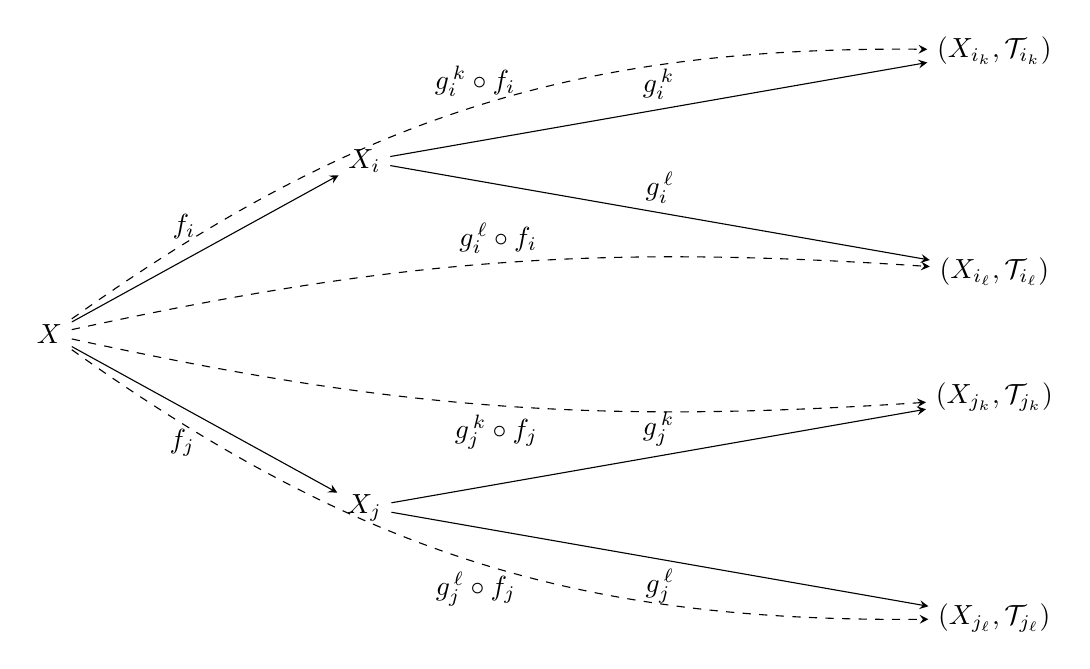
\begin{tikzpicture}[>=stealth, xscale=2, yscale=2]
% Knoten
\node (X)   at (0,0)      {$X$};

\node (Xi)  at (2,1.1)    {$X_i$};
\node (Xj)  at (2,-1.1)   {$X_j$};

\node (Xik) at (6,1.8)    {$(X_{i_k},\mathcal T_{i_k})$};
\node (Xil) at (6,0.4)    {$(X_{i_\ell},\mathcal T_{i_\ell})$};
\node (Xjk) at (6,-0.4)   {$(X_{j_k},\mathcal T_{j_k})$};
\node (Xjl) at (6,-1.8)   {$(X_{j_\ell},\mathcal T_{j_\ell})$};

% Pfeile von X zu Xi, Xj
\draw[->] (X) -- (Xi) node[midway, above left] {$f_i$};
\draw[->] (X) -- (Xj) node[midway, below left] {$f_j$};

% Pfeile Xi -> Xik/Xil
\draw[->] (Xi) -- (Xik) node[midway, above] {$g_i^{\,k}$};
\draw[->] (Xi) -- (Xil) node[midway, above] {$g_i^{\,\ell}$};

% Pfeile Xj -> Xjk/Xjl
\draw[->] (Xj) -- (Xjk) node[midway, above] {$g_j^{\,k}$};
\draw[->] (Xj) -- (Xjl) node[midway, below] {$g_j^{\,\ell}$};

% gestrichelte Außenbögen (Kompositionen)
\draw[->, dashed, bend left=18]
  (X) to node[midway, above] {$g_i^{\,k} \circ f_i$} (Xik);

\draw[->, dashed, bend left=8]
  (X) to node[midway, above] {$g_i^{\,\ell} \circ f_i$} (Xil);

\draw[->, dashed, bend right=8]
  (X) to node[midway, below] {$g_j^{\,k} \circ f_j$} (Xjk);

\draw[->, dashed, bend right=18]
  (X) to node[midway, below] {$g_j^{\,\ell} \circ f_j$} (Xjl);

\end{tikzpicture}

}

\begin{proof}
    Sei $ \langle Y, \mathcal{V} \rangle$ Topologische Räume und
    $g: \langle Y, \mathcal{V} \rangle \to \langle X, \mathcal{T} \rangle$ eine Abbildung.
    \begin{itemize}
        \item Sei $\forall i \in I \forall k \in J_k: (g_{i_\ell}\circ f_i) \circ g$ stetig.
        sei $i \in I$. Dann ist $f_i \circ g :  Y,  \to \ X_i 
        \forall \ell \in J_i : g_{i_\ell}\circ(f_i \circ g)$ stetig.
        $\Rightarrow f_i \circ g: \langle Y, \mathcal{V} \rangle \to \langle X_i, \mathcal{T}_i \rangle$ stetig.
        \\
        $g: \langle Y, \mathcal{V} \rangle \to \langle X, \mathcal{T} \rangle$ stetig.
        $ \Rightarrow g: \langle Y, \mathcal{V} \rangle \to \langle X, \mathcal{W} \rangle$ stetig.

        \item Sei $g: \langle Y, \mathcal{V} \rangle \to \langle X, \mathcal{W} \rangle$ stetig.
        $\Rightarrow \langle Y, \mathcal{V} \rangle \to \langle X_i, \mathcal{T}_i \rangle$ stetig $\forall i \in I$.
        \nt{Was da pasiert ist nix}
        $\overset{\text{Satz 11.2.2 (ii) $\Rightarrow$ (i)}}{\Longrightarrow}$ $\mathcal{T} =\mathcal{W}$

        \item[Spurtopologie] $$\langle X, \mathcal T \rangle \text{ top. Raum} Y \subseteq X$$
        $\mathcal T\!\restriction_Y = \{  O \cap Y \mid O \in \mathcal T \}$
        $$ \iota: \begin{cases}
            Y \to X\\
            y \mapsto y
        \end{cases}
        $$
        $\langle Y, \mathcal{V} \rangle 
        \overset{\iota}{\longrightarrow}
        \langle X, \mathcal{T} \rangle
        \qquad
        \text{initiale Top. v. }\mathcal{T}, \iota
        $\\
        $\mathcal{V} \text{ ist kleinste Top. auf } Y 
        \text{ mit } \supseteq\{\, \iota^{-1}(O) \mid O \in \mathcal{T} \,\}\iota^{-1}(O)$
        $O \cap Y = \iota^{-1}(O) $
        $\Rightarrow\quad \mathcal V = \mathcal T\!\restriction_Y$
        \item Sei $\langle Z, \mathcal{W} \rangle$ topologischer Raum, $g: Z \to Y$ Dann ist 
        $\langle Z, \mathcal{W} \rangle \overset{g}{\to} \langle Y, \mathcal{V} \rangle$ stetig genau dann,
        wenn $\langle Z, \mathcal{W} \rangle \overset{\iota \circ g}{\to} \langle X, \mathcal{T} \rangle$ stetig ist.
        \item $Z \subseteq Y \subseteq X$ $\langle X, \mathcal{T} \rangle$ topologischer Raum.
        \item $$
        (\mathcal T\!\restriction_Y)\!\restriction_Z
        = \{\, Q \cap Z \mid Q \in \mathcal T\!\restriction_Y \,\}
        = \Bigl\{\, 
        \underbrace{{(O \cap Y)} \cap Z}_{ = O \cap (Y \cap Z)
        = O \cap Z}= \mid O \in \mathcal T 
        \,\Bigr\}
        $$
 $$
\begin{tikzpicture}[>=latex,scale=1.25]

% Punkte "..." links und rechts
\node at (-3.2,1.2) {$\dots$};
\node at (3.2,1.2) {$\dots$};

% X_i links und rechts
\node (XiL) at (-2,1.2) {$X_i$};
\node (dots) at (0,1.2) {$\dots$};
\node (XiR) at (2,1.2) {$X_i$};

% disjunkte Vereinigung in der Mitte
\node (UX) at (0,0.3) {$\bigcup X_i$};

% Existenz + Eindeutigkeit Symbol
%\node at (0,-0.05) {$\exists !\ \Phi$};

% Y unten
\node (Y) at (0,-1.3) {$Y$};

% obere Pfeile iota_i, iota_j
\draw[->] (XiL) to[bend right=30] node[midway, left] {$\iota_i$} (UX);
\draw[->] (XiR) to[bend left=30] node[midway, right] {$\iota_j$} (UX);

% untere Bögen beta_i, beta_j
\draw[->] (XiL) to[bend right=45] node[midway, left] {$\beta_i$} (Y);
\draw[->] (UX) to node[midway] {$\exists ! \Phi$} (Y);
\draw[->] (XiR) to[bend left=45] node[midway, right] {$\beta_j$} (Y);

\end{tikzpicture}
$$      
% disjunkte Vereinigung
$$
\dot{\bigcup} X_i = \bigcup_{i\in I} (X_i \times \{i\})
$$

$$
\iota_i :\begin{cases} X_i \to \dot{\bigcup} X_i, \\
x \mapsto (x,i)
\end{cases}
$$
$$
\overline{\beta}(z) = \beta_i(x),
\qquad
\text{wobei } i, x \text{ so gewählt, dass } z = (x,i)
$$

wohldef.


\nt{Beispiel: Faltentopologie}
{
$$
\langle X, \mathcal T \rangle, \quad \sim \text{ Äquivalenzrel.}
$$

$$
\langle X, \mathcal T \rangle 
\overset{\pi}{\longrightarrow}
\langle X/{\sim},\ \mathcal T/{\sim} \rangle
$$
}

    \end{itemize}
\end{proof}

\dfn{}
{
    Seien $\langle X, \mathcal{T} \rangle$ ein topologischer Raum und $i \in I$. $X$ Menge, 
    $f_i: X \to X_i$ Abbildungen, $\forall i \in I$.
    Die \textbf{finale Topologie} $\mathcal{T}_{\text{final}}$ auf $X$ bezüglich der Familie von Abbildungen 
    $(f_i)_{i \in I}$ ist die größte Topologie auf $X$, so dass alle Abbildungen $f_i$ stetig sind.   
    $$
     \mathcal{T}_{\text{final}} := \text{Topologie erzeugt von } \bigcup_{i \in I}\{f_i(O_i) \mid O_i \in \mathcal{T}_i\} 
    $$  
}

Diese Definition ist gerechtfertigt durch da:

\mlenma{}
{
    $$\{=\in X\mid \forall i \in I: f_i^{-1}(O_i) \in \mathcal{T}_i \}$$ Ist eine Topologie auf $X$
}

\begin{proof}{Lemma 11.2.5}
    \begin{itemize}
        \item[$\bullet$] $\emptyset, X \in \mathcal{T}_{\text{final}}$ da $f_i^{-1}(\emptyset) = \emptyset$ und 
        $f_i^{-1}(X) = X$.
        \item[$\bullet$] Sei $(U_\alpha)_{\alpha \in A} \subseteq \mathcal{T}_{\text{final}}$ eine Familie.
        Dann ist 
        $$
        f_i^{-1}\Bigl(\bigcup_{\alpha \in A} U_\alpha\Bigr)
        = \bigcup_{\alpha \in A} f_i^{-1}(U_\alpha) \in \mathcal{T}_i
        $$
        $\Rightarrow \bigcup_{\alpha \in A} U_\alpha \in \mathcal{T}_{\text{final}}$.
        \item[$\bullet$] Sei $U, V \in \mathcal{T}_{\text{final}}$. Dann ist 
        $$
        f_i^{-1}(U \cap V) = f_i^{-1}(U) \cap f_i^{-1}(V) \in \mathcal{T}_i
        $$
        $\Rightarrow U \cap V \in \mathcal{T}_{\text{final}}$.
    \end{itemize}
\end{proof}
\thm{11.2.6}
{
    Seien $\langle X_i,\mathcal{T}_i \rangle,  i \in I$ topologische Räume, $X$ eine Menge und 
    $f_i: X \to X_i$ Abbildungen, $\forall i \in I$. und $\mathcal{T}$ ist Topologie auf $X$.
    Dann sind die folgenden Aussagen äquivalent:
    \begin{enumerate}
        \item[(i)] $\mathcal{T} = \mathcal{T}_{\text{final}}$
        \item[(ii)] Für jeden topologischen Raum $\langle Y, \mathcal{V} \rangle$ und jede Abbildung 
        $g: \langle X, \mathcal{T} \rangle \to \langle Y, \mathcal{V} \rangle$ ist stetig genau dann, wenn alle Kompositionen 
        $g \circ f_i: \langle X_i, \mathcal{T}_i \rangle \to \langle Y, \mathcal{V} \rangle$ stetig sind, $\forall i \in I$.
    \end{enumerate}
}
\thm{}
{
    Sei $X$ eine Menge, $\langle X_i, \mathcal{T}_i \rangle, i \in I$ topologische Räume und 
    $X_{i_k}, k\in J_i $ Mengen mit Abbildungen $f_i: X_i \to X$ für $i \in I$ und $\mathcal{T}_{i_k}$ auf 
    $X_{i_k}$. 
    Sei $\mathcal{T}_i$ die finale Topologie auf $X_i$ bezüglich der Familie von Abbildungen
    $g_{i_k}: X_{i_k} \to X_i, k \in J_i$,
    sei $\mathcal{T}$ die finale Topologie auf $X$ bezüglich der Familie von Abbildungen 
    $f_i: X_i \to X, i \in I$,
    und sei $\mathcal{W}$ die finale Topologie auf $X$ bezüglich der Familie von Abbildungen 
    $f_i \circ g_{i_k}: X_{i_k} \to X, k \in J_i, i \in I$.
    \\
    Dann gilt $\mathcal{T} = \mathcal{W}$.
}

\begin{proof}{Satz 11.2.6}\\
    \begin{itemize}
        \item["$(ii)\Rightarrow$(i)"] 
        $$
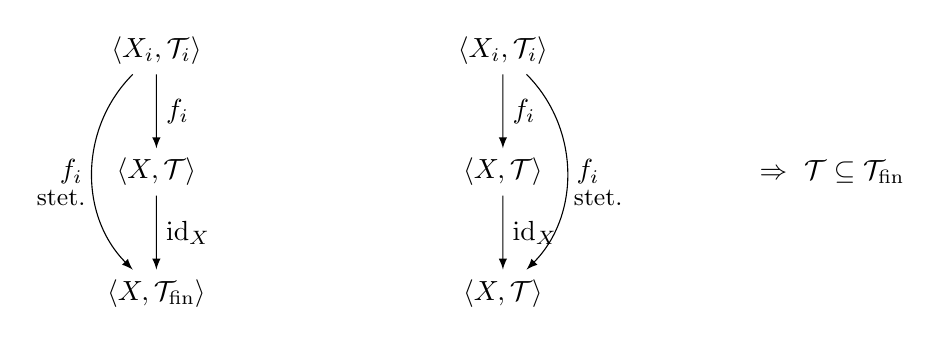
\begin{tikzpicture}[>=latex,scale=1.1]

% erstes Diagramm (links)
\node (XiL)   at (-2,1.4) {$\langle X_i,\mathcal T_i\rangle$};
\node (XT)    at (-2,0)   {$\langle X,\mathcal T\rangle$};
\node (XTfin) at (-2,-1.4){$\langle X,\mathcal T_{\mathrm{fin}}\rangle$};

\draw[->] (XiL) -- (XT)    node[midway,right] {$f_i$};
\draw[->] (XT)  -- (XTfin) node[midway,right] {$\mathrm{id}_X$};


\node at (-3.1,-0.3) {\small stet.};


% zweites Diagramm (rechts)
\node (XiR)   at (2,1.4) {$\langle X_i,\mathcal T_i\rangle$};
\node (XT2)   at (2,0)   {$\langle X,\mathcal T\rangle$};
\node (XT3)   at (2,-1.4){$\langle X,\mathcal T\rangle$};

\draw[->] (XiL) to[bend right=45] node[midway, left] {$f_i$} (XTfin);
\draw[->] (XiR) to[bend left=45] node[midway, right] {$f_i$} (XT3);

\draw[->] (XiR) -- (XT2)    node[midway,right] {$f_i$};
\draw[->] (XT2)  -- (XT3) node[midway,right] {$\mathrm{id}_X$};

\node at (3.1,-0.3) {\small stet.};


% Folgerung T \subset T_fin
\node at (5.8,0) {$\Rightarrow\ \mathcal T \subseteq \mathcal T_{\mathrm{fin}}$};

\end{tikzpicture}
$$

$$
\text{alle Beweise analog zu }\mathcal T_{\mathrm{ini}}.
$$
    \end{itemize}
\end{proof}